\documentclass[11pt]{article}
%\addbibresource{references.bib}

% custom code
\usepackage[dvipsnames]{xcolor}
\definecolor{light-gray}{gray}{0.75}
\newcommand{\code}[1]{\colorbox{light-gray}{\texttt{#1}}}

\usepackage{tikz}
\def\checkmark{\tikz\fill[scale=0.4](0,.35) -- (.25,0) -- (1,.7) -- (.25,.15) -- cycle;}  %checkmark

% images
\usepackage{graphicx}
\graphicspath{ {./img/} }

% background
\pagecolor{white}

% bibliography
\usepackage[round]{natbib}

% document links
\usepackage{hyperref}
\hypersetup{
    colorlinks,
    linkcolor={MidnightBlue!50!black},
    citecolor={MidnightBlue!50!black},
    urlcolor={MidnightBlue!80!black}
}

% tooltips
%\usepackage[inactive,blur=0.6, fixcolor]{fancytooltips}

\title{Flatland}
\author{Murphy}
\date{\today}

\begin{document}

% Title page
\maketitle	
\pagebreak

% Table of contents
\tableofcontents
\pagebreak

% Paper content

% Problem background
\section{Introduction}
\subsection{Problem Background}
The Flatland framework seeks to address the problem of automated train scheduling and rescheduling, a major challenge
for modern railway systems. It does so by providing a simplified two-dimensional grid world environment to allow for fast experimentation of new approaches to this problem \cite{monylascscbhwaegeibavistsasp20a}. 

\subsection{Related Works}
Scenarios in Flatland exist at the intersection of several well-explored problems.  At its core, Flatland is a multi-agent pathfinding problem; several agents cooperate to complete their goals while managing limited resources within a shared, finite environment.  Outside of pathfinding, Flatland is, in essence, a vehicle rescheduling problem—derived from the vehicle scheduling problem.  An understanding of how each of these problems influences Flatland is a critical piece of finding ideal methods of producing solutions.

\subsubsection{Multi-agent Pathfinding}
Multi-agent pathfinding (MAPF) is a planning problem in which agents in a shared environment must find routes to their respective destinations without incurring collisions \citep{silver05a}.  MAPF has many applications, including in robotics, aviation, and vehicle routing \citep{standley10a}.  Many of the conflicts imposed on agents in MAPF problems are also imposed on agents within the Flatland framework, such as that they may not occupy the same cell at the same time step, or that two agents may not swap positions.  These are to model collisions that would occur in real life.  

Traditional grid environments seen in many MAPF problems, including in \citep{standley10a}, have cells that are often four- or eight-connected; this means that an agent occupying one cell may move to any of its existing unoccupied neighboring cells.  The Flatland framework is more restrictive in this sense, as agents are not free to move indiscriminately to any unoccupied neighboring cell, but rather may move to neighboring cells according to transitions governed by the track type of that cell and the orientation of the agent at that time step, all of which is further discussed in \autoref{sec:Environment} and is illustrated more clearly in \autoref{fig:grids}.

% Figure: Grids, degrees of freedom
\begin{figure}[t]
\centering
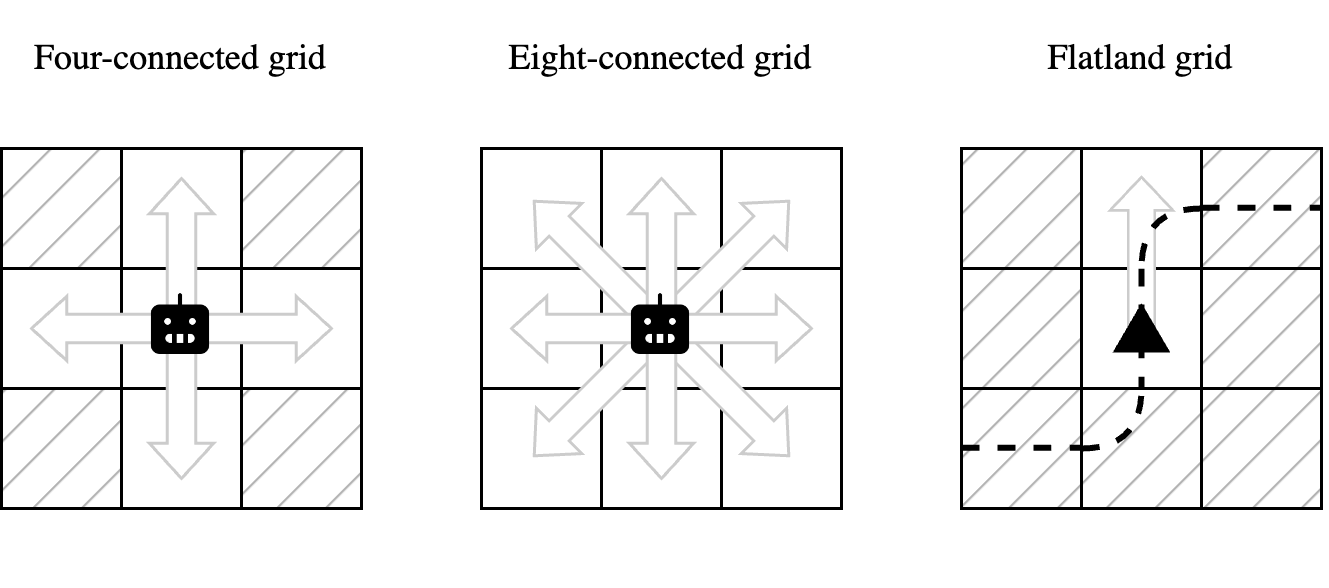
\includegraphics[width=\textwidth]{grids}
\caption{Examples of the degrees of freedom for agents in four-connected grid environments, eight-connected grid environments, and Flatland grid environments. The orientation of the agent in Flatland is necessary to determine which cells are accessible. }
\label{fig:grids}

\begin{center}
{\color{lightgray} \rule{\linewidth}{0.15mm}}
\end{center}

\end{figure}

\subsubsection{Vehicle Scheduling Problem}
The vehicle scheduling problem (VSP) is a classical optimization problem in the field of operational planning of public transportation systems, consisting of assigning vehicles to trips, in such a way that each trip is associated to one vehicle and a cost function is minimized \citep{bapeukfa00a}.  This problem has been a topic of operational research for decades, but is not the primary focus of Flatland, as each instance already provides a set of agents with pairs of starting and ending positions. Since the agents come pre-assigned to the origin and destination, the importance is shifted from assigning vehicles to trips to actively determining their paths.  However, since Flatland randomly inflicts breakdowns upon its fleet, the task effectively transforms into a vehicle rescheduling problem.

\subsubsection{Vehicle Rescheduling Problem}
The vehicle rescheduling problem (VRSP) is an extension of the VSP and arises when a previously-scheduled trip is disrupted due to interruptions such as a medical emergency or a vehicle breakdown \citep{limibo07a}.  Trips in the Flatland environment model this scenario by randomly assigning vehicle breakdowns, each of which stops a train in its current location for an unforeseen duration.  Ideally, scheduled trips that are affected by a breakdown should be rescheduled in such a way that there are minimal impacts to the original plan.  \citep{limibo07a} note the severity of this problem, in that it results not only in direct operational and delay costs for transit providers, but also in inconvenience for passengers.  The lack of automated rescheduling policies, as well as algorithms that address this problem, highlights the importance of the role that Flatland plays in focusing its scenarios on the element of rescheduling disrupted trips.


% Potential approaches
\section{Approaches}
AIcrowd hosts a global competition in which participants submit crafted approaches to scenarios in the Flatland environment, which are scored and compared against one another.  The variety of submissions highlights the diverse nature of approaches taken to solve the problem Flatland presents.

\subsection{Reinforcement Learning}
Reinforcement learning is a form of machine learning in which an agent with a goal is not told what steps to take, but rather discovers a path to it by determining which actions yield the greatest reward \citep{sutton18a}.  This differs from \textit{supervised learning} in which agents are shown a set of labeled examples of desired outcomes so that it can generalize for unseen situations.  This also differs from \textit{unsupervised learning} in which agents seek to uncover structures or patterns within a set of unlabeled examples.  A typical reinforcement learning approach in a Flatland scenario would include many iterations of agents relying on past actions that have yielded success and exploring new actions that aim to get them closer to the goal.

Although the competition is open to approaches from any domain, it has branded itself as a competition for multi-agent reinforcement learning.  In the latest two iterations of the competition, separate leaderboards were posted for those pursuing the reinforcement learning track and those pursuing all other approaches.  Despite this focus, the highest any participant has placed with a reinforcement learning solution has been seventh place.

\subsection{Operations Research}
Operations research is a broader field pertaining to the application of scientific methods to problems involving the operations of a system, such as by using the theories of probability, linear programming, queuing theory, or other methods \citep{gupta92a}.  The winners of the 2020 competition were a team led by professors Daniel Harabor and Peter J. Stuckey of Monash University.  The team employed a prioritized planning approach to quickly find collision-free paths, and a large neighborhood search (LNS) to improve the solution quality thereafter \citep{lichzhchhastmako21a}.

In each the last two competitions, teams with operations research-focused approaches have taken the top four spots.  The winning team members from 2020 explain in \citep{lichzhchhastmako21a} why they believe reinforcement learning approaches have not produced the same level of success as other methods:
\begin{itemize}
	\item reinforcement learning approaches need to predict future deadlocks, which appears difficult to determine without directly reasoning about paths, as optimization approaches do
	\item as the density of an environment grows, the number of situations that can lead to deadlocks increases non-linearly
	\item optimization approaches rely on global planners, which have been shown to consistently outperform reinforcement learning approaches across all rounds of both the 2019 and 2020 Flatland competitions
\end{itemize}


\subsection{Answer Set Programming}
Answer set programming (ASP) is a form of declarative programming, based on the stable model semantics of logic programming, oriented toward difficult search problems \citep{lifschitz19a}.  ASP has wide-ranging applications in technology and science, with a particular inclination toward NP-hard\footnotemark problems.

\footnotetext{NP-hard represents a category of problems in computer science whose answers can neither be solved quickly nor verified quickly. \textit{Quickly} is a relative term for the speed of an algorithm that can solve problems in polynomial time, a duration considered reasonably efficient.}

The pathfinding problem that is present in Flatland scenarios is, at its core, an NP-hard search problem.  ASP presents itself as a particularly suitable approach to solving pathfinding problems in Flatland for several reasons:
\begin{itemize}
	\item as a declarative language, encodings are constructed in terms of their goals, not their intermediate steps
	\item solutions are clearly characterized by their formalization, and one can clearly see the correspondence of the solution to the encoding
	\item encodings can be easily adapted to changing conditions, such as by adding more agents or including additional constraints
\end{itemize}

\noindent Generally, the flexibility, maintainability, human readability, and verifiability of ASP lends itself well to scalable pathfinding problems. \medskip

[Concerns or drawbacks about traditional machine learning methods compared to ASP]

% The problem workflow
\section{Building Blocks}
Flatland comprises a set of components that are fundamental to its ability to simulate real-world railway scenarios.  In the forefront are the environment and the agents, which form the basis of modeling how trains traverse a physical network.

Further components include the scope of observation, the presence of breakdowns, and pre-determined timetables.  However, these are not considered within the scope of this research.

\subsection{Environment}
\label{sec:Environment}
An environment in Flatland is a grid that consists of cells that are either empty or contain tracks.  A track may belong to one of nine types, and may be rotated in increments of 90º.  Cells must be arranged in such a way that they form a cohesive network, even if the resulting network is simplistic.  Each cell may only be occupied by a single agent at any given time step.

\subsubsection{Track Types and Transitions}
\label{sec:Track}
Flatland documentation considers seven track types, however, two of them have alternative representations that this paper recognizes as individual types, bringing the total to nine.  There is also a separate designation for an empty cell.  A visual representation of the track types can be seen in \autoref{fig:tracks}.

% Figure: Grids, degrees of freedom
\begin{figure}[t]
\centering
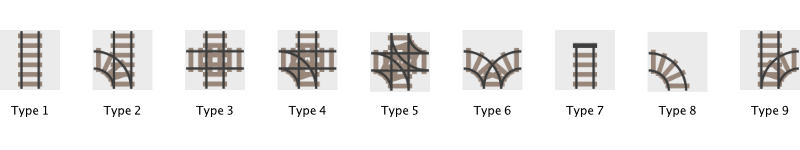
\includegraphics[width=\textwidth]{tracks}
\caption{Visual representation of all available track types.  Each type may be rotated in increments of 90º.  Type 8 and Type 9 are variations on Type 1 and Type 2, respectively, which cannot be attained through rotation alone.}
\label{fig:tracks}

\begin{center}
{\color{lightgray} \rule{\linewidth}{0.15mm}}
\end{center}

\end{figure}

The various rail types can be grouped into two categories: non-switches and switches.  Non-switches include tracks such as straight tracks, curved tracks, and dead ends.  These do not allow an agent to change the course of its path.  Conversely, switches represent decision points, as they compel agents to make a choice.  A switch will never present more than two options.

Each rail type determines the possible transitions for the agents, meaning which neighboring cells are accessible positions following a single move.  Crucially, neighboring cells that are accessible from one location, may in some cases not be accessible had the train approached this same location from another direction.  This is a fundamental underlying quality of the Flatland environment.  For this reason, recording both the position and orientation of each agents at every time step is necessary for determining its legal paths.  A diagram explaining this quality is shown in \autoref{fig:transitions}.

% Figure: Grids, degrees of freedom
\begin{figure}[t]
\centering
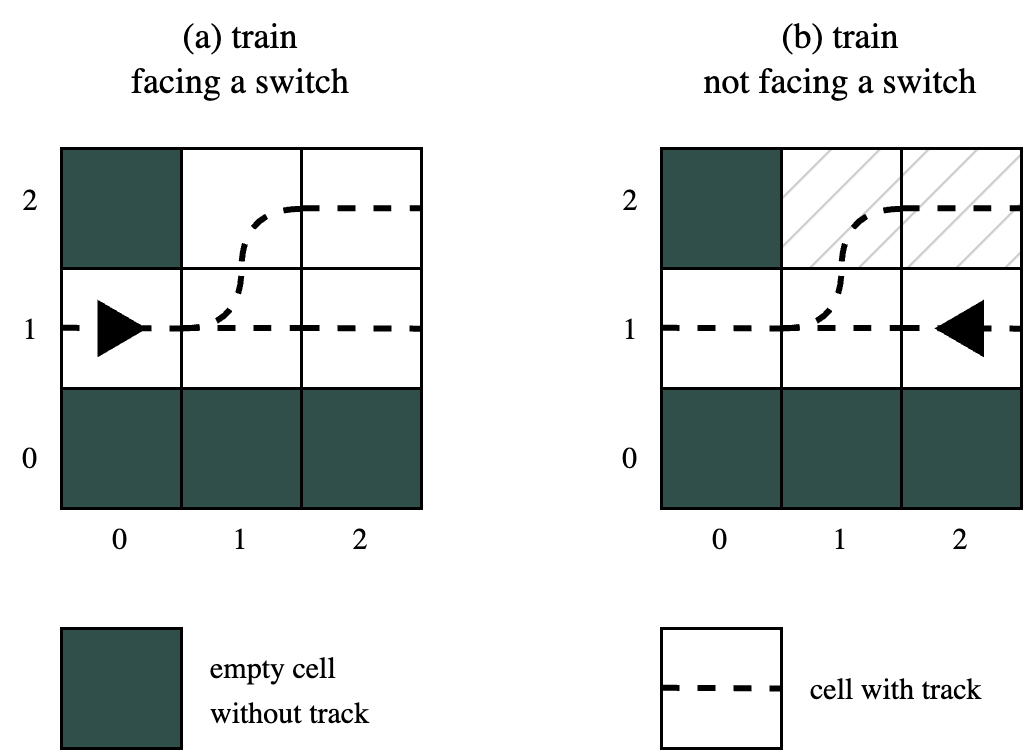
\includegraphics[width=0.60\textwidth]{transitions}
\caption{The switch on cell \texttt{(1,1)} is only accessible from one side.  In environment (a), the agent is facing east on cell \texttt{(0,1)}.  When it reaches cell \texttt{(1,1)}, it will have the option to continue to the east or follow the switch to the north.  In environment (b), the agent is facing west on cell \texttt{(2,1)} and does not have access to the switch.  Therefore, when it reaches cell \texttt{(1,1)}, it will only have the option to continue moving west.}

\begin{center}
{\color{lightgray} \rule{\linewidth}{0.15mm}}
\end{center}

\label{fig:transitions}
\end{figure}



\subsubsection{Points of Interest}
The Flatland framework offers several parameters when generating novel environments.  Namely, the \code{sparse\_rail\_generator} allows users to specify:
\begin{itemize}
	\item the number of cities
	\item the number of intersections
	\item the number of train stations
	\item the minimal distance between nodes
	\item the proximity of stations to their associated cities
	\item the number of connections between cities
\end {itemize}

\noindent From the perspective of the trains, cities play no functional role; they are purely esthetic. Train stations, however, play a crucial role, as the journey of any train may only begin and end at designated train stations.  The remaining parameters offer flexibility in defining the degree of connectedness and overall character of the track layout. \medskip


\subsection{Agents}
\label{sec:Agents}
Agents in Flatland represent the trains of a railway network.  They can choose from a set of actions, are given starting locations and specified destinations, must avoid collisions and other conflicts with agents present throughout the environment, and have various speed profiles.  The terms \textit{agent} and \textit{train} are used interchangeably.

Additionally, agents in Flatland may have different speeds, depending on their train types, such as passenger trains or freight trains.  This speed profile determines how quickly agents are capable of traversing the environment, and ultimately influences how they interact with one another.  The scope of this research recognizes only a uniform speed profile and does not distinguish between train types.  Trains in motion are capable of traversing the environment at a rate of one cell per time step.

\subsubsection{Actions}
\label{sec:Actions}
Within the environment, agents follow a series of actions.  Since Flatland is a discrete time simulation, the duration of each action conforms to a constant amount of time.    At each time step, agents must choose from one of the following five actions: 
\begin{enumerate}
  \item \code{MOVE\_FORWARD}: this action moves the train forward, provided there is a legal transition that allows this; this is also the appropriate action along curved track with no switch
  \item \code{MOVE\_LEFT}: this action moves the train along a switch to the left, provided there is a legal transition that allows this
  \item \code{MOVE\_RIGHT}: this action moves the train along a switch to the right, provided there is a legal transition that allows this
  \item \code{STOP\_MOVING}: this action stops the train, resulting in its remaining in the current cell
  \item \code{DO\_NOTHING}: this action compels the train to adhere to a continuation of its previous action; the one exception is that while stopped in a dead end, this reverses the direction of the train
\end{enumerate} \smallskip

\noindent So long as a valid action has been selected, the position and orientation of the agent will be updated in the following time step. \medskip

\begingroup

\setlength{\tabcolsep}{9pt} % Default value: 6pt
\renewcommand{\arraystretch}{1.2} % Default value: 1

\begin{table}[]
\centering
\begin{tabular}{rcccc}
                                      		& -90º 		& 0º 			& 90º 		& 180º \\
\hline % ————————————————————————————————————————
\texttt{MOVE\_FORWARD} 	& \checkmark  	& \checkmark 	& \checkmark  	& \\
\texttt{MOVE\_LEFT}    		& \checkmark 	& 			& 			& \\
\texttt{MOVE\_RIGHT}   		& 			& 			& \checkmark 	& \\
\texttt{STOP\_MOVING}  		& 			& \checkmark 	& 			& \\
\texttt{DO\_NOTHING}  	 	& \checkmark	& \checkmark	& \checkmark 	& \checkmark   
\end{tabular}
\caption{How each action can change the orientation of an agent in the following time step.  A change of 0º is analogous to no change.}
\label{tbl:actions}
\begin{center}
{\color{lightgray} \rule{\linewidth}{0.15mm}}
\end{center}
\end{table}


\endgroup

As shown in \autoref{tbl:actions}, different actions are capable of affecting subsequent agent orientation in various ways.  The typical effect that \code{MOVE\_FORWARD} imposes is no change on the agent orientation in the following time step.  The exception to this is on curved track (Type 9 in \autoref{fig:tracks}) which can rotate the agent by 90º counterclockwise or clockwise, depending on the direction of the curve.   \code{MOVE\_LEFT} and \code{MOVE\_RIGHT} will always alter the current orientation of the agent by 90º counterclockwise or clockwise, respectively.  As the \code{DO\_NOTHING} command repeats the previously-invoked action, the change in orientation would typically mimic the change of the previous action.  The notable exception to this is when the agent is in a stopped position in a dead end (Type 7 in \autoref{fig:tracks}), in which case it will reverse its direction, altering the current orientation by 180º.  \code{STOP\_MOVING} will never alter the current orientation of the agent.

\subsubsection{Starting and Ending Positions}
\label{sec:Positions}
Each agent is given a starting position and orientation, as well as a destination.  The goal for a single agent is to traverse the environment by choosing valid actions along legal paths that lead the agent from its starting position to its destination.  

For simplicity, trains are not recognized by the environment until they are actively underway.  This prevents trains who have not yet begun their journeys from occupying space on the tracks and preventing the passage of other trains.  Likewise, once a train reaches its destination, it is no longer recognized as actively being present in the environment.  The track space therefore becomes free in the time step after the train has completed its journey.

\subsubsection{Conflict Restrictions}
\label{sec:Conflicts}
Consistent with core tenets of any MAPF problem, any two trains must avoid a collision with each other.  Agents, as with trains in real life, may not physically pass through one another.  This restriction prevents one train from overtaking a stopped train on the same set of tracks; it also prevents two trains facing each other from swapping positions.

\bibliographystyle{plainnat}
\bibliography{references}
\end{document}